\chapter{Our Protocol}
	In this chapter, we describe our protocol with FSwRD approach beginning from query dissemination phase till the detecting an adversary.
	Our protocol using FSwRD can also be applied using FSwoRD with the obvious modifications. 
	We briefly describe the differences along the way.

	% If you implement FSwRD approach in real network it looks similar to this chapter. 
	% In the end, we describe the difference between FSwRD and FSwoRD as well. 

\section{Query Dissemination}
	The protocol begins with the base station initiating the query request to the sensor network.
	The base station does the authenticated broadcast of its query to the entire sensor network asking the network to report the aggregated result of the sensor reading values.
	It includes the query nonce in its query to avoid replay attacks in the future. 
	We use the same hash chain process to generate unique query nonce for the base station as described in Section \ref{sec:query-dissemination}.
	Once the sensor nodes receive the query from the base station they constructs their own leaf vertex by creating the data-items of their sensor readings and its signature.
	The sensor nodes constructs their payloads and send it to their parent in the aggregation tree. 
	The details of the commitment tree generation is described in the next section.

\section{Commitment Tree Generation}
	For the given aggregation tree the commitment forest is built as follows.
	The commitment tree generation begins from the sensor nodes with the highest depth (leaf nodes) in the aggregation tree.
	Leaf sensor nodes in the aggregation tree constructs their leaf vertices by creating data-items, signatures of those data-items and signature of the transmit-payload according to Equations \ref{eq:data-item}, \ref{eq:sign-data-item}, \ref{eq:signing-payload}, respectively.
	Then they send the payload to their parents in the aggregation tree.	
	Each internal sensor node in the aggregation tree also constructs their leaf vertex.
	In addition, internal sensor node receives the payload from each of its children, which impacts its forest.
	For each child, internal node first verifies the signature of the transmit-payload and then the signature of the data-item for one child at a time.
	Once internal node verifies all the received signatures, it merges all the data-items with same count value from its forest.
	It merges two data-items by creating a new data-item with count value incremented by one and whose value is the addition of value field of the previous two data-items. 
	Note that we can easily determine the height of the commitment tree from the count value.
	Suppose, after verifying all the signatures from the payloads, an internal sensor node $I$ has to merge $i$ data-items $D_{1}$, $D_{2}$, $\dotsc$, $D_{i}$ in its forest.
	% First, $I$ verifies all the received payload signatures.
	% Then $I$ verifies the received signatures $Sign(D_{1})$, $Sign(D_{2})$, $\dotsc$, $Sign(D_{i})$.
	% Once verified, $I$ starts merging the data-items as follows.
	Let $c$ be the smallest count value in $I$'s forest.
	The sensor node $I$ finds two data-items $D_{1}$ and $D_{2}$ from its forest with the same count value $c$ and merges them into a new data-item with the count of $c+1$ as shown in Figure \ref{fig:increase-height}.
	It repeats the process until no two data-items in its forest have the same count value.	
	The data-item of the $A_{2}$ is given as follows:
	% 
	\begin{equation*}
		A_{2} =\ <A_{id}, 4, A_{2value},H(N||4||A_{2value}||B_{1}||D_{1})>;\ A_{2value} = B_{1value} + D_{1value}. 
	\end{equation*}
	% 
	
	\begin{figure}[h!]
		% \centering
		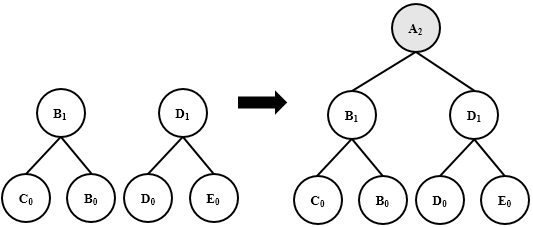
\includegraphics{images/increase-height.png}
		\caption{Input node $A$ has $B_{1}$ and $C_{1}$ in its forest. It aggregates these two trees and constructs $A_{2}$.}
		\label{fig:increase-height}
	\end{figure}
	
	We demonstrate the commitment tree generation process for the aggregation tree shown in Figure \ref{fig:Aggregation-tree-1}.
	\begin{figure}[h!]
		\centering
		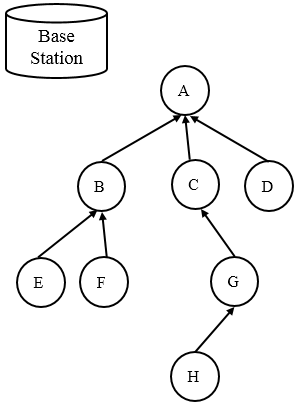
\includegraphics{images/aggregation-tree-1.png}
		\caption{Aggregation Tree.}
		\label{fig:Aggregation-tree-1}
	\end{figure}
	In this example, $A$ has three children.
	$A$ receives one payload from each of its children, which impacts $A$'s forest.
	After verifying all the signatures from each child's payload, $A$ uses the data-items in its forest to constructs its payload, which is sent to the base station.
	We describe the payload generation process for sensor nodes $B,C,D$ and $A$ in order.

	The sensor node $B$ constructs its payload from its forest. 
	It's forest consists of payloads received from $E$ and $F$.
	The leaf sensor nodes $E$ and $F$ constructs their payloads according to Equation \ref{eq:signing-payload} as follows:
	% \begin{figure}[h!]
	% 	\centering
	% 	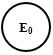
\includegraphics{images/e-payload.png}
	% 	\caption{E's payload}
	% 	\label{fig:e-payload}
	% \end{figure}

	\begin{equation*}
		\begin{array}{l}
		E_{pay} =\ <E_{0}, \textsf{Sign}_{\sk_{E}}(E_{0}), \textsf{Sign}_{\sk_{E}}(E_{\tau}) >\ where\ E_{\tau} =\ <E_{0}>\\
		E_{0} =\ <E_{id}, 1, E_{value}, H(N||1||E_{value})>\\
		F_{pay} =\ <F_{0}, \textsf{Sign}_{\sk_{F}}(F_{0}), \textsf{Sign}_{\sk_{F}}(F{\tau}) >\ where\ F_{\tau} =\ <F_{0}>\\
		F_{0} =\ <F_{id}, 1, F_{value}, H(N||1||F_{value})>.
		\end{array}
	\end{equation*}
	
	$B$ receives $E_{pay}$ and $F_{pay}$ from $E$ and $F$ respectively. 
	$B$ verifies all the signatures in the received payloads.
	Then it constructs its own data-item $B_{0}$.
	Now, $B$ has $B_{0},E_{0},F_{0}$ in its forest as shown in Figure \ref{fig:b-forest-payload}. 
	As all the data-items have the same count value, $B$ has an option while selecting two data-items to merge.
	$B$ aggregates $E_{0},F_{0}$ and constructs $B_{1}$.
	After creating $B_{1}$ none of the data-items have the same count value. 
	So, $B$ constructs its payload $B_{pay}$ and sends it to $A$ as follows:
	\begin{equation*}
		\begin{array}{l}
			B_{pay} =\ < B_{0}, \textsf{Sign}_{\sk_{B}}(B_{0}), B_{1}, \textsf{Sign}_{\sk_{B}}(B_{1}), \textsf{Sign}_{\sk_{B}}(B_{\tau}) >\ where\ B_{\tau} =\ <B_{0} || B_{1}>\\
			B_{1} =\ < B_{id}, 2, B_{1value}, H(N||2||B_{1value}||E_{0}||F_{0})>;\ B_{1value} = E_{value} + F_{value} \\
			B_{0} =\ <B_{id}, 1, B_{value}, H(N||1||B_{value})>
		\end{array}
		\label{eq:b-payload}
	\end{equation*}

	\begin{figure}[h!]
		\centering
		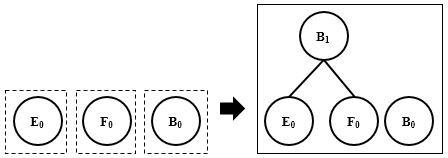
\includegraphics{images/b-forest-payload.png}
		\caption{Transformation from $B$'s forest to its payload.
				Each dashed-line box shows forest and solid-line box shows payload of the respective sensor node.}
		\label{fig:b-forest-payload}
	\end{figure}

	In similar way, the sensor node $C$ in the aggregation tree receives $G_{pay}$ from $G$ which is defined as follows:
	\begin{equation*}
		\begin{array}{l}
			G_{pay} =\ <G_{1},\textcolor{red}{\textsf{Sign}_{\sk_{G}}(G_{1})}, \textsf{Sign}_{\sk_{G}}(G_{\tau})>\ where\ G_{\tau} =\ <G_{0} || H_{0}>\\
			G_{1} =\ < G_{id}, 2, G_{1value}, H(N||2||G_{1value}||G_{0}||H_{0})>;\ G_{1value} = G_{value} + H_{value} \\
			G_{0} =\ <G_{id}, 1, G_{value}, H(N||1||G_{value})>\\
			H_{0} =\ <H_{id}, 1, H_{value}, H(N||1||H_{value})>
		\end{array}
	\end{equation*}
	$C$ verifies all the signatures in the received payload $G_{pay}$ and constructs $C_{0}$.
	Now, $C$ has $C_{0},G_{1}$ in its forest as shown in Figure \ref{fig:c-forest-payload}. 
	As none of the data-items have the same count value, $C$ does not merge those two data-items.
	But $C$ removes the old signature on $G_{1}$ and signs $G_{1}$ with its secret key.
	So, $C$ constructs its payload $C_{pay}$ and sends it to $A$ as follows:
	\begin{figure}[h!]
		\centering
		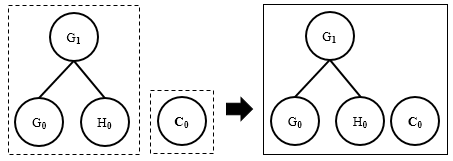
\includegraphics{images/c-forest-payload.png}
		\caption{$C$'s forest aggregation creating its payload.}
		\label{fig:c-forest-payload}
	\end{figure}
	\begin{equation*}
		\begin{array}{l}
			C_{pay} =\ <C_{0},\textsf{Sign}_{\sk_{C}}(C_{0}),G_{1},\textcolor{red}{\textsf{Sign}_{\sk_{C}}(G_{1})}, \textsf{Sign}_{\sk_{C}}(C_{\tau})>\ where\ C_{\tau} =\ <C_{0} || G_{1}>\\
			C_{0} =\ <C_{id}, 1, C_{value}, H(N||1||C_{value})>
		\end{array}
		%\label{eq:c-payload}
	\end{equation*}

	The sensor node $D$ constructs its payload $D_{pay}$ and sends it to $A$ as follows:
	\begin{equation*}
		\begin{array}{l}
			D_{pay} =\ <D_{0}, \textsf{Sign}_{\sk_{D}}(D_{0}), \textsf{Sign}_{\sk_{D}}(D_{\tau})>;\ where\ D_{\tau} =\ <D_{0}>\\
			D_{0} =\ <D_{id},1,D_{value},H(N||1||D_{value})>
		\end{array}
		%\label{eq:d-payload}
	\end{equation*}

	The root node of the aggregation tree $A$ receives the payloads $B_{pay}, C_{pay}$ and $D_{pay}$ from $B,C$ and $D$ respectively.
	% Equations \ref{eq:b-payload},\ref{eq:c-payload},\ref{eq:d-payload} 
	$A$ verifies all the signatures in the received payloads and constructs $A_{0}$.
	Now, $A$ has $G_{1},C_{0},B_{1},B_{0},D_{0}$ and $A_{0}$ in its forest as shown in Figure \ref{fig:a-forest}.
	\begin{figure}[h!]
		\centering
		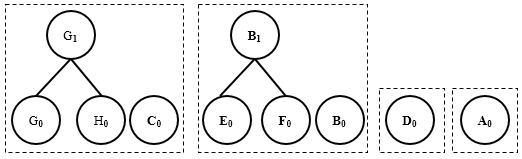
\includegraphics{images/a-forest.png}
		\caption{$A$'s forest: $A$ receives three payloads from $C,B,D$ and constructs $A_{0}$}
		\label{fig:a-forest}
	\end{figure}
	\begin{figure}[h!]
		\centering
		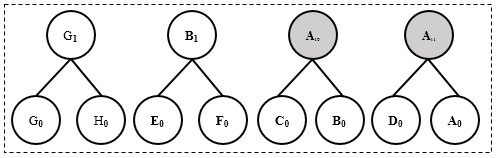
\includegraphics{images/a-forest-first-merge.png}
		\caption{$A$'s forest: after first merge}
		\label{fig:a-forest-first-merge}
	\end{figure}
	\begin{figure}[h!]
		\centering
		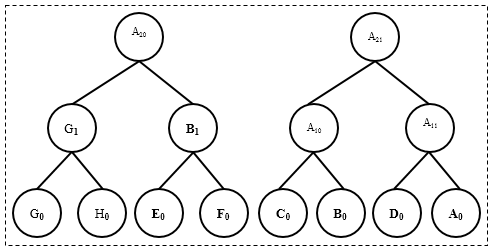
\includegraphics{images/a-forest-second-merge.png}
		\caption{$A$'s forest: after second merge}
		\label{fig:a-forest-second-merge}
	\end{figure}
	$A$ has four data-items with count value of $1$.
	In the first merge, $A$ aggregates those data-items and constructs $A_{10}$ and $A_{11}$ as shown in Figure \ref{fig:a-forest-first-merge}.
	Now, $A$ has four data-items with count value of $2$.
	In the second merge, $A$ aggregates those data-items and constructs $A_{20}$ and$A_{21}$ as shown in Figure \ref{fig:a-forest-second-merge}.
	Finally, $A$ has two data-items with count value of $4$.
	In the final merge, $A$ aggregates those data-items and constructs $A_{3}$ as shown in Figure \ref{fig:a-payload}.
	Then $A$ constructs payload and sends it to the base station as follows:
	% 		
		\begin{equation*}
			\begin{array}{l}
				A_{pay} =\ <A_{3},\textsf{Sign}_{\sk_{A}}(A_{3}),\textsf{Sign}_{\sk_{A}}(A_{\tau})>\ where\ A_{\tau} =\ <A_{3}>\\
				A_{3} =\ <A_{id}, 8, A_{3value}, H(N||8||A_{3value}||A_{20}||A_{21})>;\ A_{3value} =\ A_{20value} + A_{21value}\\
				A_{20} =\ <A_{id},4,A_{20value},H(N||4||A_{20value}||G_{1}||B_{1})>;\ A_{20value} =\ G_{1value} + B_{1value}\\ 
				A_{21} =\ <A_{id},4,A_{21value},H(N||4||A_{21value}||A_{10}||A_{11})>;\ A_{21value} =\ A_{10value} + A_{11value}\\ 
				A_{10} =\ <A_{id},2,A_{10value},H(N||2||A_{10value}||B_{0}||C_{0})>;\ A_{10value} =\ B_{value} + C_{value}\\
				A_{11} =\ <A_{id},2,A_{11value},H(N||2||A_{11value}||D_{0}||A_{0})>;\ A_{11value} =\ D_{value} + A_{value}\\
				A_{0} =\ <A_{id},1,A_{value},H(N||1||A_{value})>
			\end{array}
		\end{equation*}
	% 
	\begin{figure}[h!]
		\centering
		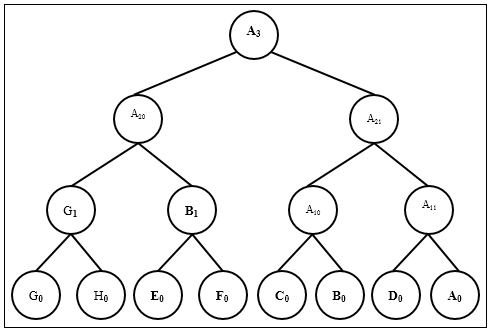
\includegraphics{images/a-payload.png}
		\caption{$A$'s payload : $A$ sends this to the base station.}
		\label{fig:a-payload}
	\end{figure}

	Once the base station receives the payload from the root of the aggregation tree, it verifies all the signatures in the payload.
	In the previous example, the base station receives $A_{pay}$ from the sensor node $A$.
	It verifies the signatures $\textsf{Sign}_{\sk_{A}}(A_{3})$, $\textsf{Sign}_{\sk_{A}}(A_{\tau})$ in the received payload.	 
	If the base station verifies all the signatures to true it initiates the result checking phase.

\section{Result Checking}
	The purpose of the \textit{result checking} phase is to require that all the sensor nodes verify their individual contributions to the final aggregate value.
	If there is any inconsistency in the aggregation process then with the help of the base station, trace down the node responsible for causing the inconsistency in the aggregation process.

	\subsection{Dissemination of Final Payload by the Base Station}
		Once the base station receives the payloads of the root node of the aggregation tree, it verifies all the signatures in the payload and then sends each of the data-items in the payload to the entire sensor network using authenticated broadcast.
		The authenticated broadcast allows the sensor nodes to verify that the data-items are sent by the base station. 
		The authentication ensures no one else is masquerading the base station.
		In our previous example, the base station receives only one data-item $A_{3}$ in the payload sent by $A$.
		In that case, the base station's payload $\textsf{B}_{pay}$ which is sent to the entire network is given as follows:
		
	 		\begin{equation*}
				\textsf{B}_{pay} =\ <A_{3}, \textsf{Sign}_{\sk_{\textsf{B}}}(A_{3}), \textsf{Sign}_{\sk_{\textsf{B}}}(\textsf{B}_{\tau})>\ where\ \textsf{B}_{\tau} =\ <A_{3}>.
			\end{equation*}
		
	\subsection{Dissemination of Off-Path Values}
		To enable verification each sensor node must receive all of its off-path values.
		The off-path values of the sensor nodes can be determined according to the Definition \ref{def:off-path}.
		Each internal vertex $I$ in the commitment tree has two children $u_{1}$ and $u_{2}$. 
		To disseminate off-path values, $I$ sends the data-item of $u_{1}$ to $u_{2}$, and vice-versa ($I$ also attaches relevant information tagging $u_{1}$ as the right child and $u_{2}$ as the left child) along with the signatures of the data-item and the signature of the transmit-payload.
		In our previous example, internal vertex $A_{10}$, shown in Figure \ref{fig:a-payload}, has two children $C_{0}$ and $B_{0}$.
		$A_{10}$ (which is sensor node $A$ in aggregation tree) sends the following off-path values to $C$ and $B$ respectively as follows:
			\begin{equation*}
				\begin{array}{l}
					<B_{0}, \textsf{Sign}_{\sk_{A}}(B_{0}),\textsf{Sign}_{\sk_{A}}(A_{\tau})>\ where\ A_{\tau} =\ <B_{0}>\\
					<C_{0}, \textsf{Sign}_{\sk_{A}}(C_{0}),\textsf{Sign}_{\sk_{A}}(A_{\tau})>\ where\ A_{\tau} =\ <C_{0}>.
				\end{array}
			\end{equation*}
		
		An internal vertex $I$ receives data-items with their respective signatures from its parent. 
		It verifies the signatures of the received data-items then resigns them and sends those data-items (and left/right tags) with their signatures to both of its children.
		Continuing the previous example, internal vertex $A_{10}$ receives $A_{11}$ and $A_{20}$ from its parent $A_{21}$.
		$A_{10}$ sends the following off-path values to $C$ and $B$ respectively as follows:
		\begin{equation*}
			\begin{array}{l}
				<B_{0}, \textsf{Sign}_{\sk_{A}}(B_{0}),A_{11},\textsf{Sign}_{\sk_{A}}(A_{11}),A_{20},\textsf{Sign}_{\sk_{A}}(A_{20}),\textsf{Sign}_{\sk_{A}}(A_{\tau})>\\
					\textcolor{white}{XXXXX}where\  A_{\tau} =\ <B_{0}||A_{11}||A_{20}>\\
				<C_{0}, \textsf{Sign}_{\sk_{A}}(C_{0}),A_{11},\textsf{Sign}_{\sk_{A}}(A_{11}),A_{20},\textsf{Sign}_{\sk_{A}}(A_{20}),\textsf{Sign}_{\sk_{A}}(A_{\tau})>\\ 
					\textcolor{white}{XXXXX}where\  A_{\tau} =\ <C_{0}||A_{11}||A_{20}>.
			\end{array}
		\end{equation*}
		
		In FSwRD, all the leaf vertices need to know only one certificate as they receive data-items signed by their parent vertex.
		In FSwoRD, all the leaf vertices might need to know $\log l$ certificates, where $l$ is the number of leaf-vertices in commitment tree including the leaf vertex.
		Continuing the previous example, $C$ and $B$ receive three signatures from $A_{10}$. 
		All these three signatures are signed by $A$.
		Hence, $C$ and $B$ need to know the certificate of $A$.  
		Whereas in FSwoRD, $C$ and $B$ receives three signatures from $A$.
		From those three two will be signed by $A$ and one will be signed by either $B$ or $C$ depending on the data-item. 
		Therefore, $B$ need to know the certificates of $A$ and $C$, and $C$ need to know the certificates of $A$ and $B$.

		We show the significance of the commitment field while distributing the off-path values. 
		The commitment filed helps us detecting any \textit{malicious activity} in the network. 
		Because of the signatures infrastructure eventually we can detect an adversary. 
		For example, if an internal vertex simply forwards incorrect data-item to its children then the relevant leaf vertex will complain, as the leaf vertex will not be able to derive the data-item received using authenticated broadcast from the base station.
		Because of the signatures internal vertex responsible for forwarding the incorrect data-item will be caught.
		Another scenario could be that an internal vertex changed the its children's data-item while creating commitment tree and sending the incorrect off-path values to compensate discrepancy. 
		To illustrate the scenario consider the following Example.

		\begin{exmp}
			\label{ex1:malicious-activity}
			Suppose the vertices in the commitment tree of Figure \ref{fig:malicious-activity} have the data-items defined as follows.
			Note that we did not include the signatures of these data-items in this example for simplification.
			\begin{equation*}
				\begin{array}{l}
					A_{0} =\ <A_{id},1,10, H(N||1||10)>\\
					B_{0} =\ <B_{id},1,20, H(N||1||20)>\\
					C_{1} =\ <C_{id},2,30, H(N||2||30||A_{0}||B_{0})>
				\end{array}
			\end{equation*}

			\begin{figure}[t]
				\centering
				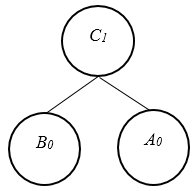
\includegraphics{images/commitment-tree-2.png}
				\caption{Smallest Possible Commitment Tree}
				\label{fig:malicious-activity}
			\end{figure}

			Now suppose $C$ changes $A_{0}$ and $B_{0}$ to $A'_{0}$ and $B'_{0}$ by changing the value fields and then applies aggregate commit algorithm.
			$C$ can send either $C'_{1}$ or $C''_{1}$ to the base station.
			But it  will be caught by base station in both cases.
			To compensate for the discrepancy, $C$ constructs $B''_{0}$ and $A''_{0}$ off-path values trying to hide its malicious activity from the base station.

			\begin{equation*}
				\begin{array}{l}
					A'_{0} =\ <A_{id},1,100, H(N||1||10)>\\
					B'_{0} =\ <B_{id},1,200, H(N||1||20)>\\
					\\
					C'_{1} =\ <C_{id},2,300, H(N||2||300||\mathbf{A''_{0}}||\mathbf{B_{0}})>\ or \\ 
					C''_{1} =\ <C_{id},2,300, H(N||2||300||\mathbf{A_{0}}||\mathbf{B''_{0}})>\\
					\\
					B''_{0} = <B_{id},1,290,H(N||1||20)>\\
					A''_{0} = <A_{id},1,280,H(N||1||10)>
				\end{array}
			\end{equation*}

			During the dissemination of the root data-item phase, $A$ and $B$ using authenticated broadcast receives either $C'_{1}$ or $C''_{1}$ from the base station based on what $C$ has sent to base station.
			During the dissemination of off-path values phase, $A$ and $B$ receives $B''_{0}$ and $A''_{0}$ from $C$ respectively.
			During the verification of inclusion phase, $A$ and $B$ derives the root data-item using the received off-path values, and it does not match with the received root data-item as follows:
			\begin{equation*}
				\begin{array}{l}
					A\ \mbox{uses}\ (A_{0}, B''_{0})\ \mbox{and derives} <2,300,H(N||2||300||\mathbf{A_{0}}||\mathbf{B''_{0}})>\  = C''_{1} \neq C'_{1} \\
					B\ \mbox{uses}\ (A''_{0}, B_{0})\ \mbox{and derives} <2,300,H(N||2||300||\mathbf{A''_{0}}||\mathbf{B_{0}})>\  = C'_{1} \neq C''_{1}.
				\end{array}
			\end{equation*}
			Hence, during the collection of authentication codes phase, either $A$ or $B$ sends its authentication codes with NACK message.
		\end{exmp}
			Above example shows how the commitment field in the data-item provides \textbf{data-integrity} to the protocol.
			It makes it nearly impossible for an adversary to tamper with the data-items while creating commitment tree and/or while distributing off-path values.
			This malicious activity can be detected by the commitment filed in the data-item.
			Later, we show that the adversary can be detected with the provided signature infrastructure.
			Once a vertex has received all the off-path vertices, it can proceed to the verification step.
	
	\subsection{Verification of Inclusion}
	
		Once the sensor node has received all the data-items of its off-path vertices from its parent, first it verifies the signature of all the received data-items and then it verifies that no aggregation result tampering has occurred on the path between its leaf vertex and the root of its commitment tree.
		It also verifies that its senor reading was aggregated correctly by all the intermediate aggregate nodes.
		For each vertex on the path from the root of its commitment tree, it derives the data-items according to Definition \ref{def:label}.
		It is able to do so since the off-path values provide all the necessary information to perform the data-item computation.
		In the previous example, $C$ receives $B_{0}, A_{11}$ and $ A_{20}$ from its parent node and it has $C_{0}$.
		It aggregates $<C_{0}, B_{0}>$ and derives $A_{10}$.
		Then it aggregates $<A_{10},A_{11}>$ and derives $A_{21}$.
		Finally it aggregates $<A_{21}, A_{20}>$ and derives $A_{3}$.
		Then it compares the derived $A_{3}$ with the $A_{3}$ received from the base station.
		Based on those data-items are identical or not the node proceeds with the next step accordingly.
		If those data-items are identical then the node sends the authentication code with ACK message and if those data-items are not identical then the node sends the authentication code with NACK message.

	\subsection{Collection of Authentication Codes}
		\label{subsection:collection-of-authentication-codes}
		The authentication codes for sensor node $I$, with their positive and negative acknowledgment message, are defined as follows:
		\begin{equation}
			\begin{array}{l}
				\mbox{Positive : } \mbox{MAC}_{\sk_{I}}(\mbox{N} || \mbox{ACK})\\
				\mbox{Negative : } \mbox{MAC}_{\sk_{I}}(\mbox{N} || \mbox{NACK})
			\end{array}
		\end{equation}

		$\sk_{I}$ is the secret key of the sensor node $I$, ACK and NACK are special messages for positive and negative acknowledgment respectively.
		The authentication code with ACK message is sent by the sensor node if it verifies its contribution correctly to the root commitment value during the \textit{verification of inclusion} phase and vice versa.
		Leaf sensor nodes in the aggregation tree first send their authentication codes to their parents in the aggregation tree.
		Once an internal sensor node has received authentication codes from all its children, it computes the XOR of its own authentication code with all the received codes, and forwards it to its parent.
		For example, the sensor node $B$ shown in Figure \ref{fig:Aggregation-tree-1}, receives the authentication codes $\mbox{MAC}_{\sk_{E}}(\mbox{N}||\mbox{ACK})$, $\mbox{MAC}_{\sk_{F}}(\mbox{N}||\mbox{ACK})$ from $E,F$ respectively, and it has its own authentication code with ACK message then $B$ sends the following authentication code to $A$.
		\begin{equation*}
			\mbox{MAC}_{\sk_{E}}(\mbox{N}||\mbox{ACK}) \oplus \mbox{MAC}_{\sk_{F}}(\mbox{N}||\mbox{ACK}) \oplus \mbox{MAC}_{\sk_{B}}(\mbox{N}||\mbox{ACK})
		\end{equation*}
		Because of the XOR function we do not have to forward all the authentication codes. 
		At the end of the process, the base station receives a single authentication code $\Delta_{root}$\ from the root of an aggregation tree.
		% We can forward only one authentication code to the base station in the end, which consume the less bandwidth in the network.
		% Note that this phase is similar to the SHIA's collection of confirmation phase.

	\subsection{Verification of Authentication Codes}
		\label{sec:verficiation-of-authentication-codes}
		
		To verify that every sensor node has sent its authentication code with \ack, the base station computes the $\Delta_{ack}$ as follows:
		\begin{equation}
			\label{eq:mac-auth}
			\displaystyle{\Delta_{ack} = \bigoplus_{i = 1}^n \mbox{MAC}_{\sk_{i}}(\mbox{N} || \mbox{ACK}) }
		\end{equation}
		Here, the addition represents an XOR operation.
		The base station can compute $\Delta_{ack}$ as it knows the secret key $\sk_{i}$\ for each sensor node $i$.
		Then it compares the computed $\Delta_{ack}$\ with the received root authentication code $\Delta_{root}$. 
		If those two codes match then it accepts the aggregated value or else it proceeds further to find an adversary. 

		To detect an adversary, the base station needs to identify which nodes in the aggregation tree sent its authentication codes with \nack\ during the verification of inclusion phase.
		The node who sent authentication code with \nack\ during the verification of inclusion phase is called a \complainer. 
		We claim that if there is a single complainer in the aggregation tree during the verification of inclusion phase then the base station can find the complainer in \textbf{linear time}.
		To find a complainer, the base station computes the complainer code $c$ as follows:
		\begin{equation}
			\label{eq:complainer}
			c := \Delta_{root} \oplus \Delta_{ack}
		\end{equation}
		Then it computes the complainer code $c_{i}$\ for all node $i = 1, 2, \dotsc, n$. 
		\begin{equation}
			\label{eq:caomplainer-node}
			c_{i} := \mbox{MAC}_{\sk_{i}}(\mbox{N} || \mbox{ACK}) \oplus \mbox{MAC}_{\sk_{i}}(\mbox{N} || \mbox{NACK})
		\end{equation}
		After that, it compares $c$\ with all $c_{i}$\ one at a time. 
		The matching code indicates the complainer node.
		The base station needs to do $C_{(n,1)}$ \footnote{$C_{(n,1)}$ = $n \choose 1 $ = $n$} calculations according to Equation \ref{eq:caomplainer-node} and same number of comparisons to find a complainer in the aggregation tree. 
		Hence, the base station can find a single complainer in linear time.
		\begin{exmp} 
			If there are four nodes ${s_{1},s_{2},s_{3},s_{4}}$ in an aggregation tree and their authentication codes with \ack, \nack\ message in the binary format are defined as follows:
			\begin{equation*}
				\begin{array}{l}
					\mbox{MAC}_{\sk_{1}}(\mbox{N}\ ||\ \mbox{ACK}) = (1001)_{2};\ \mbox{MAC}_{\sk_{1}}(\mbox{N}\ ||\ \mbox{NACK}) = (1101)_{2}\\
					\mbox{MAC}_{\sk_{2}}(\mbox{N}\ ||\ \mbox{ACK}) = (0110)_{2};\ \mbox{MAC}_{\sk_{2}}(\mbox{N}\ ||\ \mbox{NACK}) = (1111)_{2}\\	
					\mbox{MAC}_{\sk_{3}}(\mbox{N}\ ||\ \mbox{ACK}) = (0101)_{2};\ \mbox{MAC}_{\sk_{3}}(\mbox{N}\ ||\ \mbox{NACK}) = (0111)_{2}\\
					\mbox{MAC}_{\sk_{4}}(\mbox{N}\ ||\ \mbox{ACK}) = (0011)_{2};\ \mbox{MAC}_{\sk_{4}}(\mbox{N} || \mbox{NACK}) = (1110)_{2}
				\end{array}
			\end{equation*}
			Suppose the root of an aggregation tree computed the $\Delta_{root} = (0100)_{2}$ as described in Subsection \ref{subsection:collection-of-authentication-codes}.
			The base station calculates $\Delta_{ack} = (1001)_{2}$ according to the Equation \ref{eq:mac-auth}.
			Then it calculates the complainer code $c = (1101)_{2}$ according to the Equation \ref{eq:complainer}.
			The base station also computes the complainer codes for each sensor node according to the Equation \ref{eq:caomplainer-node} as follows:
			\begin{equation*}			
				c_{1} = (0100)_{2}, c_{2} = (1001)_{2}, c_{3} = (0010)_{2}, c_{4} = (1101)_{2}
			\end{equation*}
			The base station compares complainer code $c$ with individual complainer code $c_{i}$ and finds that $c=c_{4}$.
			So, the base station identifies that the $s_{4}$\ complained, during verification of inclusion phase.
		\end{exmp}
		The following binary illustration helps visualize that applying XOR is negating the contribution of the authentication code with NACK.
		The base station receives the following from the root an aggregation tree, which includes one authentication code with NACK.
		\[
			\underbrace{			
				\begin{array}{cccc}
					1 & 0 & 0 & 1 \\ 
					0 & 1 & 1 & 0 \\
					0 & 1 & 0 & 1 \\
					1 & 1 & 1 & 0 \\
					\hline
					0 & 1 & 0 & 0 
				\end{array}
				}_{\Delta_{root}}
		\]
		The base station calculates $\Delta_{ack}, \Delta_{nack} $ and complainer code $c$ as follows:
		\[ 
			\underbrace{
				\begin{array}{ccccc}
					& 1 & 0 & 0 & 1 \\ 
					& 0 & 1 & 1 & 0 \\
					& 0 & 1 & 0 & 1 \\
					+ & 0 & 0 & 1 & 1 \\
					\hline
					 & 1 & 0 & 0 & 1 
				\end{array}
			}_{\Delta_{ack}}
			\mbox{          }
			\underbrace{
				\begin{array}{cccc}
					1 & 1 & 0 & 1 \\ 
					1 & 1 & 1 & 1 \\
					0 & 1 & 1 & 1 \\
					1 & 1 & 1 & 0 \\
					\hline
					1 & 0 & 1 & 1 
				\end{array}
		}_{\Delta_{nack}}			
		\]
		\[ 
			\underbrace{
			\begin{array}{cccc}
				1 & 0 & 0 & 1 \\ 
				0 & 1 & 0 & 0 \\
				\hline
				1 & 1 & 0 & 1 \\
			\end{array}
		}_{c}		
		\]
		Then the base station calculates the complainer code for each node $i$ as follows:
		\[
			\underbrace{
				\begin{array}{cccc}
				1 & 0 & 0 & 1\\
				1 & 1 & 0 & 1\\
				\hline
				0 & 1 & 0 & 0\\
				\end{array}
			}_{c_{1}}
			\mbox{   }
			\underbrace{
				\begin{array}{cccc}
				0 & 1 & 1 & 0\\
				1 & 1 & 1 & 1\\
				\hline
				1 & 0 & 0 & 1\\
				\end{array}
			}_{c_{2}}
			\mbox{   }
			\underbrace{
				\begin{array}{cccc}
				0 & 1 & 0 & 1\\
				0 & 1 & 1 & 1\\
				\hline
				0 & 0 & 1 & 0\\
				\end{array}
			}_{c_{3}}
			\mbox{   }
			\underbrace{
				\begin{array}{cccc}
				0 & 0 & 1 & 1 \\
				1 & 1 & 1 & 0 \\
				\hline	
				1 & 1 & 0 & 1\\
				\end{array}
			}_{c_{4}}
		\]
		% \[
		% 	\begin{array}{cccc    cccc    cccc    cccc}
		% 		1 & 0 & 0 & 1\ \vline\  0 & 1 & 1 & 0\ \vline\  0 & 1 & 0 & 1\ \vline\  0 & 0 & 1 & 1 \\
		% 		1 & 1 & 0 & 1\  \vline\ 1 & 1 & 1 & 1\ \vline\	0 & 1 & 1 & 1\ \vline\	1 & 1 & 1 & 0 \\ 
		% 		\hline
		% 		0 & 1 & 0 & 0\  \vline\ 1 & 0 & 0 & 1\ \vline\ 0 & 0 & 1 & 0\ \vline\ 1 & 1 & 0 & 1\\
		% 	\end{array}
		% \]
		Finally, concludes that node $4 $ is complaining.
		
		In general, to find $k$\ complainers the base station needs to do $C_{(n,k)}$ \footnote{$C_{(n,k)}$ = $ n \choose k$ = $n!/(k! \cdot (n-k)!)$} calculations and the same number of comparisons to find $k$\ complainers.
		Suppose, there are more than one complainer in the network then the base station uses the following recursive algorithm to find all the complainers in the network.
		
		\begin{algorithm}
			\caption{Finding complainer tree in a given forest}
			\label{algo:detect-a-complainer-tree}
			\begin{algorithmic}[1]
				\STATE BS requests authentication codes of all the tree roots in the aggregation tree root's forest.
				\STATE BS simulates authentication codes of all the tree roots in the aggregation tree root's forest with ACK message.
				\STATE BS compares the requested and simulated authentication codes.
				\STATE BS constructs \textsf{T} = $\{\textsf{T}_{1},\textsf{T}_{2},\dotsc,\textsf{T}_{n}\}$ whose authentication codes do not match.
				\FORALL {$t \in \textsf{T}$}
					\STATE Call Algorithm \ref{algo:detect-a-complainer} with ($t$)			
				\ENDFOR 
			\end{algorithmic}
		\end{algorithm}

		\begin{algorithm}
			\caption{Finding complainer node in a given tree}
			\label{algo:detect-a-complainer}
			\begin{algorithmic}[1]
				\STATE BS requests the authentication codes of each child $C_{1}$ and $C_{2}$ of the given tree.
				\STATE BS simulates the authentication codes of the given tree's each child with ACK message.
				\STATE BS compares the requested and simulated authentication codes and identifies $C'$ whose authentication codes do not match.
				\IF {$C'$ is a leaf vertex}
					\STATE Add $C'$ to \sf{C} 
				\ELSE
					\STATE Call Algorithm \ref{algo:detect-a-complainer} with ($C'$)			
				\ENDIF
			\end{algorithmic}
		\end{algorithm}
		Note the fact that, in Algorithm \ref{algo:detect-a-complainer}, one of the child nodes will not match with the simulated authentication codes of the base station.
		These algorithms are recursive and runs in exponentially time.
		This algorithm detects complainers faster if there are more complainers in the same commitment tree.
		Hence, we expect this algorithm to run in linear time.

	\subsection{Detecting An Adversary}
		Once the base station finds the node who sent NACK during the verification of inclusion phase, it interacts with the nodes in the network to trace an adversary responsible for it. 
		The base station tries to constructs a set of possible adversaries based on a set of possible cheaters.
		The following example demonstrates that if the base station knows the commitment tree topology and the complainers in the network then it can guess the possible adversaries.
		For simplicity, we selected the commitment tree where all the vertices are unique. 
		This analysis holds true for any commitment tree topology. 
		\begin{exmp}
			The base station constructs a set $\textsf{C} =\{\textsf{C}_{1},\textsf{C}_{2} , \dotsc, \textsf{C}_{n}\}$ for the complainers based on the protocol described in the Section \ref{sec:verficiation-of-authentication-codes}.
			Then based on the set $\textsf{C}$ it constructs a set $\textsf{A} = \{\textsf{A}_{1},\textsf{A}_{2},\dotsc,\textsf{A}_{n}\}$ of the possible adversaries. 
			\begin{figure}[t]
				\centering
				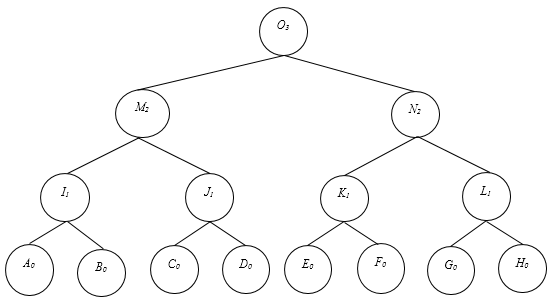
\includegraphics{images/possible-cheaters.png}
				\caption{A Commitment Tree With All Unique Vertices}
				\label{fig:cheating}
			\end{figure}

			Suppose $\textsf{C}=\{A_{0}\}$ then a possible set of adversary $\textsf{A} =\{I,\{B,I\},\{B,M\},\{B,I,M\}\}$. 
			Note the fact that only $I$ knows the exact data-item of $A_{0}$. 
			The vertices $M$ and $O$ knows aggregated value of $A_{0}$. 
			Hence, if either $M$ or $O$ tampers they tamper with more than one data-item or they have to cheat in a group. 
			Based on the fact that the possible set of adversaries for given complainer set are as follows:\\
			If $\textsf{C}=\{A_{0},B_{0}\}$ then $\textsf{A}=\{I,M,\{I,M\},\{C,D,O\}\}$\\
			If $\textsf{C}=\{A_{0},B_{0},C_{0}\}$ then $\textsf{A}=\{\{D,O\},\{I,J\},\{M,J\},\{M,J,I\}\}$\\				
			If $\textsf{C}=\{A_{0},B_{0},C_{0},D_{0}\}$ then $\textsf{A}=\{M, O,\{I,J\},\{E,F,G,H,O\}\}$\\			
			If $\textsf{C}=\{A_{0},B_{0},C_{0},D_{0},E_{0}\}$ then $\textsf{A}=\{\{O,K\},\{M,K\},\{J,I,K\},\{F,G,H,O\}\}$\\				
			If $\textsf{C}=\{A_{0},B_{0},C_{0},D_{0},E_{0},F_{0}\}$ then $\textsf{A}=\{\{O,K\},\{M,N\},\{N,O\},\{J,I,K\}\}$\\
			If $\textsf{C}=\{A_{0},C_{0}\}$ then $\textsf{A}= \{ \{J,I\}\}$
		\end{exmp}

		Now, we describe the case for detecting an adversary for a single complainer case.
		In above example, if $c = {A_{0}}$ then $a=\{I,\{B,I\},\{B,M\},\{B,I,M\}\}$.
		Suppose $I$ is an adversary and it changed the $A_{0}$ to $A'_{0}$, creating an internal vertex $I'_{1}$ instead of $I_{1}$ while creating the commitment tree. 
		Then,
		\begin{equation*}
			\begin{array}{l}
				I_{1} =\ <I_{id}, 1, I_{1value}, H(N||1||I_{value}||A_{0}||B_{0})> \mbox{where}\ I_{1value} = A_{value} + B_{value}\\	
				I_{pay} = <I_{1}, \textsf{Sign}_{\sk_{I}}(I_{1}), \textsf{Sign}_{\sk_{I}}(I_{\tau})> \mbox{where}\ I_{\tau} = I_{1}\\
			\end{array}
		\end{equation*}
		Whereas,
		\begin{equation*}
			\begin{array}{l}
				I'_{1} =\ <I_{id}, 1, I'_{1value}, H(N||1||I'_{value}||A'_{0}||B_{0})> \mbox{where}\ I_{1value} = A'_{value} + B_{value}\\
				I'_{pay} = <I'_{1}, \textsf{Sign}_{\sk_{I}}(I'_{1}), \textsf{Sign}_{\sk_{I}}(I_{\tau})> \mbox{where}\ I_{\tau} = I'_{1},\\
			\end{array}
		\end{equation*}
		To detect an adversary, first the base station asks $A$ to send its payload.
		\begin{equation*}
			\begin{array}{l}
			A_{pay} = <A_{0}, \textsf{Sign}_{\sk_{A}}(A_{0}), \textsf{Sign}_{\sk_{A}}(A_{\tau})> \mbox{where}\ A_{\tau} = A_{0}\\
			A_{0} = <A_{id}, 1, A_{value}, H(N||1||A_{value})>
			\end{array}
		\end{equation*}
		Then the base station asks $I$ to send all the received payloads from each of its children and its own payload.
		So, $I$ instead of sending the its true payload it sends its false payload to the base station.
		As $I$ is an adversary it might lie about it and send the following payload.
		\begin{equation*}
			\begin{array}{l}
				A_{pay} = <A_{0}, \textsf{Sign}_{\sk_{A}}(A_{0}), \textsf{Sign}_{\sk_{A}}(A_{\tau})> \mbox{where}\ A_{\tau} = A_{0}\\
				B_{pay} = <B_{0}, \textsf{Sign}_{\sk_{B}}(B_{0}), \textsf{Sign}_{\sk_{A}}(B_{\tau})> \mbox{where}\ B_{\tau} = B_{0}\\
				I_{pay} = <I_{1}, \textsf{Sign}_{\sk_{I}}(I_{1}), \textsf{Sign}_{\sk_{A}}(I_{\tau})> \mbox{where}\ I_{\tau} = I_{0}\\
			\end{array}
		\end{equation*}
		Then the base station asks $M$ to send all the received payload from each of its children.
		So, $M$ sends the following to the base station.
		\begin{equation*}
			\begin{array}{l}
				I'_{pay} = <I'_{1}, \textsf{Sign}_{\sk_{I}}(I'_{1}), \textsf{Sign}_{\sk_{I}}(I_{\tau})> \mbox{where}\ I_{\tau} = I'_{1}\\
				J_{pay} = <J_{1}, \textsf{Sign}_{\sk_{I}}(J_{1}), \textsf{Sign}_{\sk_{A}}(J_{\tau})> \mbox{where}\ J_{\tau} = J_{0}\\
			\end{array}
		\end{equation*}
		As the base station receives the $I'_{pay}$ with a signature from $M$, then this proves that the $I$ has lied about its payload.
		Hence, $I$ is an adversary.
		In general, the bases station utilizes the following algorithm to trace an adversary.
		\begin{algorithm}
			\caption{Pseudo algorithm to detect an adversary}
			\label{algo:detect-an-adversary}
			\begin{algorithmic}[1]

				\STATE BS\ identifies all the complainer and constructs $\textsf{C} = \{\textsf{C}_{1}, \textsf{C}_{2}, \dotsc, c\textsf{C}_{n}\}$
				\FORALL {$C \in \textsf{C}$}

					\STATE BS asks $C$ to send data-item with its signature, sent during commitment tree generation phase
				
				\ENDFOR

				\STATE BS identifies possible adversary based on $\textsf{C}$ and constructs $\textsf{A} = \{\textsf{A}_{1},\textsf{A}_{2},\dotsc,\textsf{A}_{n}\}$

				\FORALL {$A \in \textsf{A}$}

					\STATE BS asks $A$ to send data-items with its signature, received and sent by $A$ during commitment tree generation phase
					\STATE If needed BS  asks the parent of $A$ to send data-items with its signature
		
				\ENDFOR

				\STATE BS determines the adversary based on the verification of signatures

			\end{algorithmic}
		\end{algorithm}

		As the adversaries tempers with the data-item, it reduces the data-integrity of the protocol.
		Once the base station detects adversaries it dispels them from the network for all the future queries.
		Doing so removes un-necessary communication for debugging purpose in the future which saves bandwidth and increases the life-time of the network.

		% Talk About Impact.